%%%% CAPÍTULO 3 - METODOLOGIA

\chapter{Metodologia}
\label{cap:metodologia}

Este capítulo aborda as metodologias de modelagem e desenvolvimento utilizadas no trabalho.

\section{Escopo do sistema}
\label{sec:escopoDoSistema}

O sistema \textit{Virtual Lab} deve possibilidar a criação e gerenciamento de instâncias de máquinas virtuais para uso em laboratórios remotos de ensino e pesquisa.
O acesso deve ser feito por meio de um navegador de internet, permitindo a utilização de qualquer dispositivo com um navagador de internet com acesso à rede.

O sistema deve acomodar dois tipos de usuários: usuários comuns e administradores.
Os usuários comuns devem ter permissão de criar instâncias de máquinas virtuais com base em templates pré-definidos, gerenciar suas próprias instâncias, bem como o conteúdo instalado nas mesmas.
Os administradores devem ter as mesmas permissões dos usuários comuns, além de gerenciar os templates de instância, controlar o acesso dos usuários comuns ao sistema e aos recursos de hardware.

O sistema deve permitir o acesso aos usuários através de autenticação por meio de usuário e senha, bem como através de um provedor de identidade externo, caso o ambiente de uso do sistema já possua um provedor de identidade.

Inicialmente, um usuário administrador deve criar os templates de instância indicando o sistema operacional e a quantidade de armazenamento disponível.
Os usuários comuns devem então criar instâncias com base nesses templates, escolhendo entre os tipos de hardware permitidos.

Ao ser criada, a instância deve passar por um processo de configuração inicial para garantir que o sistema operacional esteja pronto para uso, e então ser disponibilizada para o usuário, que poderá acessá-la atráves da página de conexões do sistema. As instâncias devem ser encerradas automaticamente após um período de inatividade.

\section{Modelagem}
\label{sec:modelagemDoSistema}

O processo de modelagem do sistema partiu de alguns princípios elementares para a construção de um sistema de software: 

\begin{itemize}
    \item \textbf{Objetividade}: Criar apenas modelos que sejam necessários para a compreensão do sistema. Modelos em excesso tornam o processo de desenvolvimento mais complexo e custoso.

    \item \textbf{Facilidade de alteração}: Os modelos devem ser fáceis de serem alterados, de forma que as mudanças no sistema possam ser refletidas rapidamente nos modelos. Esse princípio é de extrema importância tanto para a extensibilidade do sistema quanto para o isolamento dos componentes em cenários de teste.

    \item \textbf{Arquitetura do sistema em primeiro lugar}: Na concepção dos componentes do sistema, é importante considerar a arquitetura do sistema como um todo, de forma que os componentes sejam coesos e acoplados de forma apropriada. Esse princípio também é relevante quando pensamos na utilização de serviços de computação em nuvem, que possuem características próprias de arquitetura, infraestrutura, segurança e modelo de cobrança.

    \item \textbf{Componentes funcionalmente independentes}: Os componentes do sistema devem ser independentes entre si, isso não significa que eles não possam se comunicar, mas que o nível de encapsulamento deve entregar funcionalidades claras e bem definidas.

    \item \textbf{Consistência das informações em todos os níveis}: As informações que são transmitidas entre os componentes do sistema devem ser verificadas e validadas em todos os níveis, garantindo que a integridade do sistema seja mantida.

\end{itemize}

O processo de modelagem do sistema foi dividido nas seguintes etapas: levantamento de requisitos, projeto de arquitetura e projeto de componentes \citep{pressman2016}.

\subsection{Levantamento de Requisitos}
\label{subsec:levantamentoDeRequisitos}

% especificação dos requisitos funcionais e não funcionais, e casos de uso

Inicialmente, os requisitos do sistema foram identificados a partir de discussões recorrentes com o orientador do trabalho, que possui experiência em desenvolvimento de sistemas de software e em ambientes de ensino e pesquisa. Além disso, é um dos responsáveis pelo gerenciamento dos recursos de infraestrutura da \gls{utfpr} servidos em nuvem publica através da \gls{aws}.

Os requisitos foram divididos em funcionais e não funcionais, e como uma forma de orientar o desenvolvimento, foram criados casos de uso para representar as interações entre os usuários e o sistema.

As Tabelas \ref{tab:requisitosFuncionaisDoSistema} e \ref{tab:requisitosNaoFuncionaisDoSistema} apresentam os requisitos funcionais e não funcionais do sistema, respectivamente.

\begin{longtable}{@{\extracolsep{\fill}}l p{.8\textwidth}}%% Ambiente longtable
\caption{Requisitos funcionais do sistema\label{tab:requisitosFuncionaisDoSistema}} \\%% Legenda e rótulo
\toprule
\textbf{Identificador} & \textbf{Descrição} \\
\midrule
\endfirsthead%% Encerra cabeçalho da primeira página
\caption[]{Requisitos funcionais do sistema} \\%% Legenda
\multicolumn{2}{r}{\textbf{(continuação)}} \\
\toprule
\textbf{Identificador} & \textbf{Descrição} \\
% \midrule
\endhead%% Encerra cabeçalho das demais páginas
% \midrule
\multicolumn{2}{r}{\textbf{(continua)}} \\
\endfoot%% Encerra rodapé das demais páginas
% \bottomrule
\\[-0.5\linha]
\caption*{\nomefonte: Autoria própria (2024)} \\
\endlastfoot%% Encerra rodapé da última página

RF01 & Deve haver três tipos de permissões de usuário no sistema: \gls{upen}, \gls{ucom} e \gls{uadm} \\ \hline

RF02 & O usuário deve ser capaz de registrar-se no sistema utilizando um e-mail válido, senha e nome de usuário \\ \hline

RF03 & O usuário deve ser capaz de autenticar-se no sistema utilizando um e-mail válido e senha \\ \hline

RF04 & O usuário deve ser capaz de autenticar-se no sistema utilizando um provedor de identidade externo \\ \hline

RF05 & O usuário deve ser capaz de encerrar a sessão no sistema \\ \hline

RF06 & O usuário deve ser capaz de confirmar seu endereço de e-mail \\ \hline

RF07 & O usuário deve ser capaz de ver suas informações de perfil \\ \hline

RF08 & O usuário deve ser capaz de visualizar as suas cotas de uso no sistema \\ \hline

RF09 & Tanto o \gls{ucom} quanto o \gls{uadm} devem ser capazes de criar instâncias com base em templates de instância e suas cotas de uso disponíveis \\ \hline

RF10 & Tanto o \gls{ucom} quanto o \gls{uadm} devem ser capazes de listar de forma paginada as instâncias que possuem \\ \hline

RF11 & Tanto o \gls{ucom} quanto o \gls{uadm} devem ser capazes de visualizar detalhes, como estado e recursos, das instâncias que possuem \\ \hline

RF12 & Tanto o \gls{ucom} quanto o \gls{uadm} devem ser capazes de excluir instâncias que possuem \\ \hline

RF13 & Tanto o \gls{ucom} quanto o \gls{uadm} devem ser capazes de ligar instâncias desligadas que possuem \\ \hline

RF14 & Tanto o \gls{ucom} quanto o \gls{uadm} devem ser capazes de desligar instâncias ligadas que possuem \\ \hline

RF15 & Tanto o \gls{ucom} quanto o \gls{uadm} devem ser capazes de reiniciar instâncias ligadas que possuem \\ \hline

RF16 & Tanto o \gls{ucom} quanto o \gls{uadm} devem ser capazes de acessar as instâncias ligadas que possuem \\ \hline

RF17 & O \gls{uadm} deve ser capaz de listar de forma paginada todos os templates de instância disponíveis \\ \hline

RF18 & O \gls{uadm} deve ser capaz de criar templates de instância \\ \hline

RF19 & O \gls{uadm} deve ser capaz de editar templates de instância \\ \hline

RF20 & O \gls{uadm} deve ser capaz de excluir templates de instância \\ \hline

RF21 & O \gls{uadm} deve ser capaz de criar templates de instância a partir de suas instâncias \\ \hline

RF22 & O \gls{uadm} deve ser capaz de listar de forma paginada todos os usuários do sistema \\ \hline

RF23 & O \gls{uadm} deve ser capaz de editar a permissão de usuários do sistema \\ \hline

RF24 & O \gls{uadm} deve ser capaz de alterar a cota de uso de usuários do sistema \\ \hline

RF25 & O usuário deve ser capaz de visualizar as notificações enviadas pelo sistema \\ \hline

RF26 & O sistema deve ser capaz de enviar notificações para os usuários alertando sobre a mudança de estado de suas instâncias \\ \hline

RF27 & O sistema permitir o uso de filtros pré-definidos e busca textual para todos os recursos de listagem \\ 

RF28 & O sistema deve ser capaz de desligar automaticamente instâncias ociosas \\ \hline

RF29 & O sistema deve forcener uma lista de imagens de sistema operacional recomendadas para a criação de templates de instância \\ \hline

RF30 & O usuário deve ser capaz de acessar a documentação do sistema \\ \hline

\end{longtable}

\begin{longtable}{@{\extracolsep{\fill}}l p{.8\textwidth}}%% Ambiente longtable
\caption{Requisitos não funcionais do sistema\label{tab:requisitosNaoFuncionaisDoSistema}} \\%% Legenda e rótulo
\toprule
\textbf{Identificador} & \textbf{Descrição} \\
\midrule
\endfirsthead%% Encerra cabeçalho da primeira página
\caption[]{Requisitos não funcionais do sistema} \\%% Legenda
\multicolumn{2}{r}{\textbf{(continuação)}} \\
\toprule
\textbf{Identificador} & \textbf{Descrição} \\
% \midrule
\endhead%% Encerra cabeçalho das demais páginas
% \midrule
\multicolumn{2}{r}{\textbf{(continua)}} \\
\endfoot%% Encerra rodapé das demais páginas
% \bottomrule
\\[-0.5\linha]
\caption*{\nomefonte: Autoria própria (2024)} \\
\endlastfoot%% Encerra rodapé da última página

RNF01 & O sistema deve ser responsivo e acessível em dispositivos móveis, mesmo que algumas funcionalidades sejam limitadas \\ \hline

RNF02 & O sistema deve ser capaz de lidar com um grande número de usuários simultâneos \\ \hline

RNF03 & O sistema deve ser capaz de lidar com um grande número de instâncias simultâneas \\ \hline

RNF04 & O sistema deve atualizar as informações do estado das instâncias em tempo real, sem técnicas de \textit{polling}\footnote{O \textit{polling} é uma técnica utilizada para acompanhar o status de uma operação baseada na execução de requisições espaçadas por um intervalo de tempo pré-definido. Essa técnica pode ser custosa e esgotar os recursos do sistema}. \\ \hline

RNF05 & O sistema deve ser capaz de lidar com a criação de instâncias em menos de 5 minutos \\ \hline

RNF06 & O sistema deve apresentar eventuais erros de forma clara e objetiva \\ \hline

RNF07 & O sistema deve sinalizar ao usuário enquanto realiza operações assíncronas \\ \hline

RNF08 & O sistema deve tratar uma conexão como ativa com uma instância se a mesma estiver sendo feita a partir do sistema. Caso contrário, a instância será considerada ociosa \\ \hline

RNF09 & A documentação do sistema deve ser clara e objetiva, contendo explicações tanto sobre o funcionamento do sistema quanto sobre a utilização do sistema, além de apresentar todos os \textit{endpoints} da API \\ \hline

\end{longtable}

\subsection{Projeto de Arquitetura}
\label{subsec:projetoDeArquitetura}
% Organização dos componentes.

Em seguida, o projeto de arquitetura do sistema foi elaborado a fim de produzir representações de alto nível dos componentes do sistema e das camadas de dado e serviço \citep{pressman2016}.

A apresentação do projeto de arquitetura foi construída utilizando o modelo de visualização de arquitetura de sistemas \textit{C4}, que promove uma abordagem que parte de uma visão abstrata do sistema, passando por visões de contexto, \textit{containers} e componentes, até chegar à visão de código \citep{brown2018}.

A figura \autoref{fig:diagramaC4ContextoDoSistema} apresenta o diagrama de contexto do sistema, que mostra as interações do sistema com os atores externos, como os usuários e o provedor de identidade externo. Esse diagrama é a ponto de partida inicial para uma visão geral do contexto, onde o sistema em si é representado como um bloco central.

\begin{figure}[H]
%\captionsetup{width=0.55\textwidth}%% Largura da legenda
\caption{Diagrama C4: Contexto do Sistema}
\label{fig:diagramaC4ContextoDoSistema}
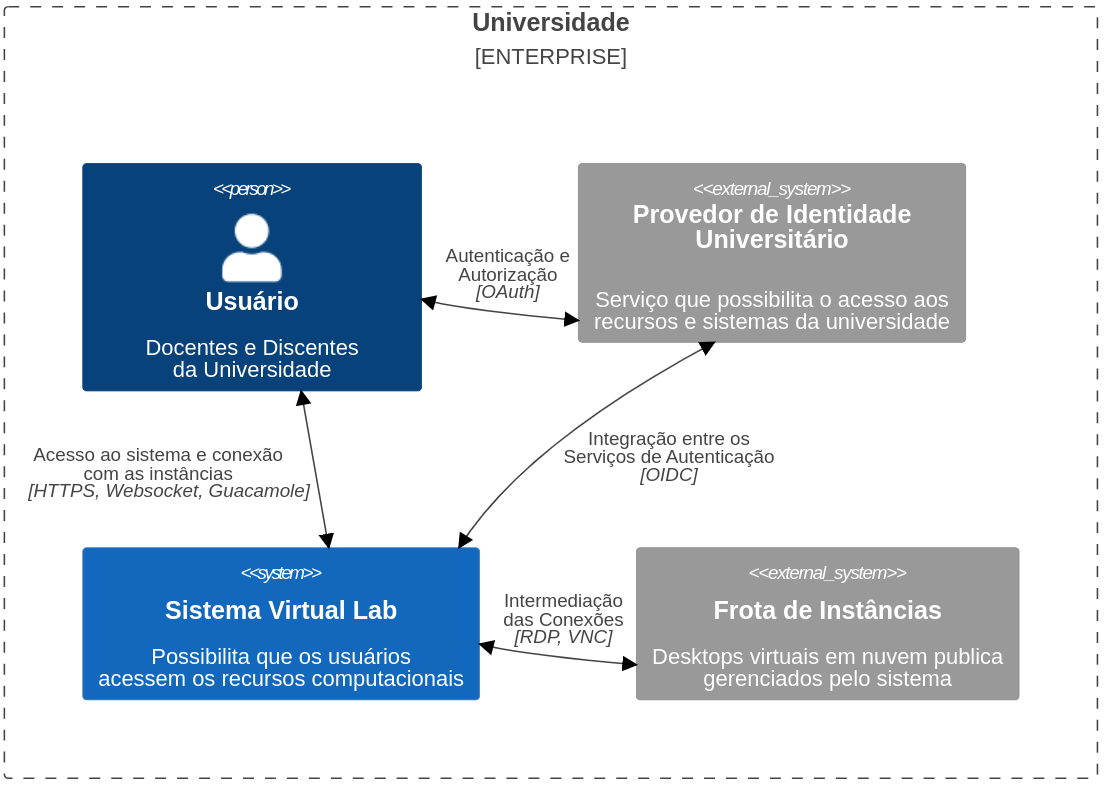
\includegraphics[width=\textwidth]{capitulos/2-metodologia/files/c4-system-context.png}
\fonte{Autoria Própria (2024)}
\end{figure}

Com uma ideia bem definida de como o sistema interage com o ambiente externo, o próximo passo foi a definição dos \textit{containers}, que são os componentes de alto nível que compõem o sistema, além de explicitar os protocolos de comunicação. O diagrama da \autoref{fig:diagramaC4ConteineresDoSistema} representa o resultado dessa etapa.

\begin{figure}[H]
%\captionsetup{width=0.55\textwidth}%% Largura da legenda
\caption{Diagrama C4: \textit{containers} do Sistema}
\label{fig:diagramaC4ConteineresDoSistema}
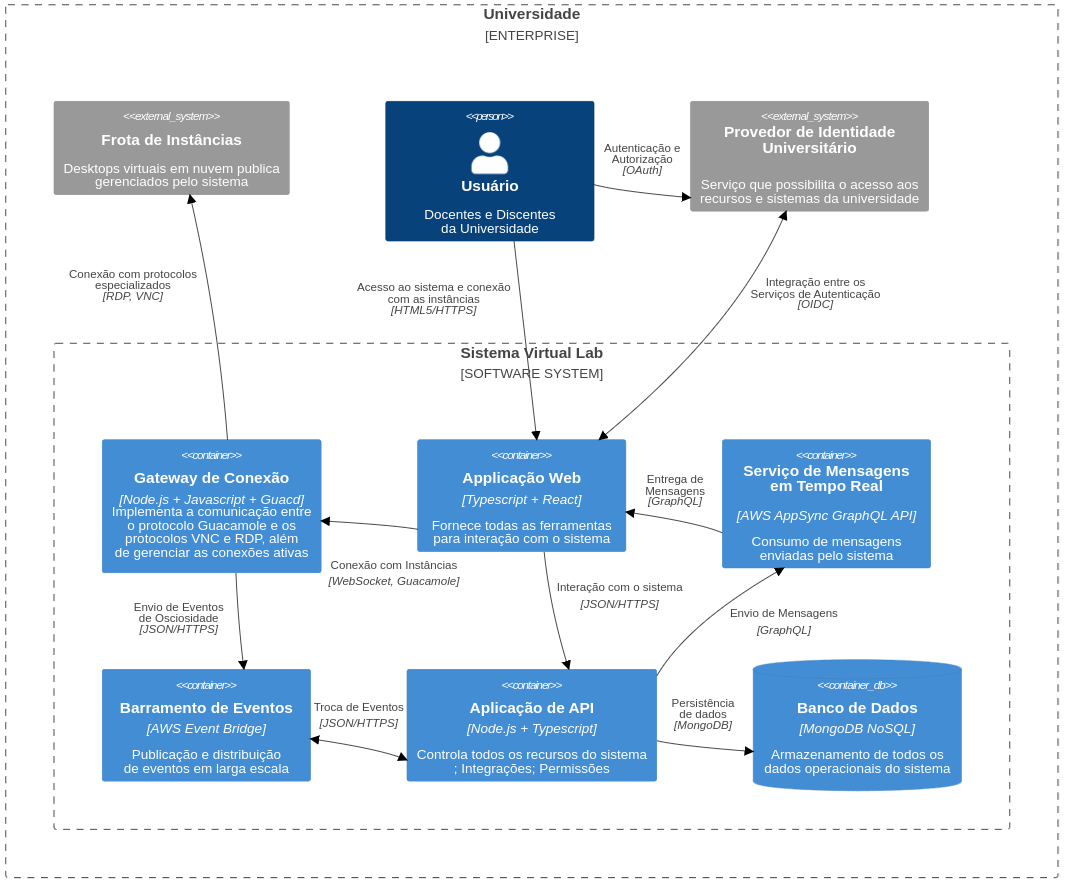
\includegraphics[width=\textwidth]{capitulos/2-metodologia/files/c4-container.png}
\fonte{Autoria Própria (2024)}
\end{figure}

A partir do diagrama de \textit{containers} do sistema, foi possível a estruturação interna de cada \textit{container} em componentes, que são as partes fundamentais para a implementação do sistema.
Nessa etapa, foram criados dois diagramas de componentes, um para a aplicação de API e outro para o gateway de conexão, que são os elos principais do sistema, representados nas figuras \autoref{fig:diagramaC4ComponentesDaAPI} e \autoref{fig:diagramaC4ComponentesDoGateway}, respectivamente.


\subsection{Projeto de Componentes}
\label{subsec:projetoDeComponentes}
% 

diagrama de componentes, diagrama de sequencia, diagrama de classes


\section{Ferramentas e Tecnologias}
\label{sec:ferramentasETecnologias}

A \autoref{tab:ferramentasETecnologiasUtilizadas} apresenta uma lista de ferramentas, tecnologias e serviços utilizados na implementação do sistema. As versões utilizadas estão escritas de acordo com o padrão de versionamento semântico. \citep{semverdocs}

% Make de last column to be as wide as possible wrapping the text
\begin{longtable}{p{0.25\linewidth} p{0.15\linewidth} p{0.525\linewidth}}%% Ambiente longtable
\caption{Ferramentas e tecnologias utilizadas\label{tab:ferramentasETecnologiasUtilizadas}} \\%% Legenda e rótulo
\toprule
\textbf{Nome} & \textbf{Versão} & \textbf{Descrição} \\
\midrule
\endfirsthead%% Encerra cabeçalho da primeira página
\caption[]{Ferramentas e tecnologias utilizadas} \\%% Legenda
\multicolumn{3}{r}{\textbf{(continuação)}} \\
\toprule
\textbf{Nome} & \textbf{Versão} & \textbf{Descrição} \\
% \midrule
\endhead%% Encerra cabeçalho das demais páginas
% \midrule
\multicolumn{3}{r}{\textbf{(continua)}} \\
\endfoot%% Encerra rodapé das demais páginas
% \bottomrule
\\[-0.5\linha]
\caption*{\nomefonte: Autoria própria (2024)} \\
\endlastfoot%% Encerra rodapé da última página
Node.js \citep{nodejsdocs} & \textsuperscript{$\wedge$}18.19.0 & Ambiente de execução de javascript utilizado em todos os serviços de backend \\

\hline

ECMAScript \citep{ecmascriptdocs} & ES2020 & Especificação formal da linguagem javascript a qual o código escrito é compatível \\

\hline

Typescript \citep{typescriptdocs} & {$\leq$}5.4.0 & Extensão do Javascript que adiciona suporte para tipagem, utilizada na implementação de todos os serviços de backend e do cliente web do sistema \\

\hline

NPM \citep{npmdocs} & 10.2.3 & Gerenciador de dependências do Node.js \\

\hline

Shell Script \citep{shellscriptdocs} & \gls{n/a} & Linguagem de scripts utilizada para implementar a configuração automatizada das instâncias baseadas em LINUX \\

\hline

Windows PowerShell Script \citep{windowspowershelldocs} & 5 & Linguagem de scripts utilizada para implementar a configuração automatizada das instâncias baseadas em WINDOWS \\

\hline

Apache Velocity Template Language \citep{apachevelocitydocs} & 2.3 & Engine de templates utilizada para definir as permissões de conexão dos usuários ao serviços de notificações do servidor ao cliente \\

\hline

Markdown \citep{markdowndocs} & \gls{n/a} & Linguagem de marcação de texto utilizada na documentação do sistema \\

\hline

OpenAPI \citep{openapidocs} & 3.0.0 & Especificação para documentação de API. \\

\hline

Zod \citep{zoddocs} & \textsuperscript{$\wedge$}3.23.8 & Biblioteca utilizada para validar o conteúdo das requisições dos serviços \\

\hline

Prettier \citep{prettierdocs} & \textsuperscript{$\wedge$}3.3.1 & Utilitário utilizado para garantir a estilização do código. \\

\hline

Jest \citep{jestdocs} & \textsuperscript{$\wedge$}29.7.0 & Framework de teste para javascript \\

\hline

Eslint \citep{eslintdocs} & \textsuperscript{$\wedge$}8.56.0 & Utilitário de análise estática de código. \\

\hline

AWS CDK \citep{awscdkdocs} & 2.142.1 & Framework utilizado para definição dos componentes de infraestrutura como código \\

\hline

SST \citep{sstdocs} & 2.43.0 & Framework para construção de aplicações full-stack na AWS utilizando infraestrutura como código \\

\hline

Docusaurus \citep{docusaurusdocs} & \textsuperscript{$\wedge$}3.4.0 & Gerador de documentação em formato de site estático. \\

\hline

React \citep{reactdocs} & \textsuperscript{$\wedge$}18.0.0 & Biblioteca utilizada no desenvolvimento do cliente web do sistema \\

\hline

Stoplight Elements \citep{stoplightdocs} & \textsuperscript{$\wedge$}8.3.1 & Biblioteca utilizada para renderização da documentação da API. \\

\hline

Docker \citep{dockerdocs} & 24.0.5 & Ferramenta utilizada para a criação do ambiente isolado do gateway de conexão \\

\hline

Chakra UI \citep{chakrauidocs} & \textsuperscript{$\wedge$}2.8.2 & Biblioteca de componentes de interface utilizada no cliente web. \\

\hline

Apache Guacamole \citep{apacheguacamoledocs} & 1.5.3 & Utilizado para intermediar a conexão entre o cliente web e gateway de conexão. \\

\hline

Vite \citep{vitedocs} & \textsuperscript{$\wedge$}5.0.12 & Ferramenta responsável por gerenciar a implementação e o empacotamento do cliente web \\

\hline

MongoDB Atlas \citep{mongodbatlasdocs} & sdk \textsuperscript{$\wedge$}6.0.3 & Serviço de banco de dados não relacional utilizado para armazenar todos os dados do sistema. \\

\hline

AWS Amplify \citep{awsamplifydocs} & sdk \textsuperscript{$\wedge$}6.0.16 & Biblioteca com integrações facilitadas, uitilizada no cliente web para autenticação e conexão com AWS AppSync \\

\hline

AWS Lambda PowerTools \citep{awslambdapowertools} & \textsuperscript{$\wedge$}2.1.1 & Biblioteca utilizada para integrar a geração de logs dos serviços com o AWS CloudWatch \\

\hline

AWS AppSync \citep{awsappsync} & sdk \textsuperscript{$\wedge$}3.592.0 & Serviço utilizado para a comunicação em tempo real entre os serviçoes de backend e o cliente web \\

\hline

AWS Systems Manager \citep{awssystemsmanagerdocs} & sdk \textsuperscript{$\wedge$}3.592.0 & Serviço utilizado para armazenar as configurações do sistema. \\

\hline

AWS Event Bridge \citep{awseventbridgedocs} & sdk \textsuperscript{$\wedge$}3.592.0 & Serviço de gerenciamento de eventos utilizado como barramento de comunicação entre os serviços de backend. Oferece também a funcionalidade de agendamento de eventos, utilizado no sistema de desligamento automático de instâncias osciosas. \\

\hline

AWS CloudFormation \citep{awscloudformationdocs} & sdk \textsuperscript{$\wedge$}3.592.0 & Serviço utilizado para armazenar a definição dos componentes de infraestrutura como código \\

\hline

AWS Cognito \citep{awscognito} & sdk \textsuperscript{$\wedge$}3.592.0 & Serviço de gerenciamento de usuários e credenciais. Ele foi utilizado para gerenciar dados sensíveis, mantendo somente dados operacionais na integração com o banco de dados. \\

\hline

AWS Service Catalog \citep{awsservicecatalogdocs} & sdk \textsuperscript{$\wedge$}3.592.0 & Serviço de gerenciamento de modelos de IaC utilizado para o controle do ciclo de vida da instância e seus recursos dependentes \\

\hline

AWS CloudWatch \citep{awscloudwatchdocs} & sdk \textsuperscript{$\wedge$}3.592.0 & Serviço de monitoramento utilizado para agregar os logs dos sistemas. \\

\hline

AWS Lambda \citep{awslambdadocs} & sdk \textsuperscript{$\wedge$}3.592.0 & Serviço de computação serverless utilizado para executar o serviço de API e tratamento de eventos do sistema \\

\hline

AWS Api Gateway \citep{awsapigatewaydocs} & sdk \textsuperscript{$\wedge$}3.592.0 & Serviço gerenciado para criação de APIs serverless. \\

\hline

AWS Identity and Access Management \citep{awsiamdocs} & sdk \textsuperscript{$\wedge$}3.592.0 & Serivço utilizado para delimitação de todas as permissões atreladas aos componentes de infraestrutura do sistema \\

\hline

AWS S3 \citep{awss3docs} & sdk \textsuperscript{$\wedge$}3.592.0 & Serviço de armazenamento de objetos utilizado para servir o cliente web e armazenar todos os arquivos imutaveis do sistema \\

\hline

AWS CloudFront \citep{awscloudfrontdocs} & sdk \textsuperscript{$\wedge$}3.592.0 & Serviço de distribuição de conteúdo utilizado como camada distribuída de cache para os serviços \\

\hline

AWS Certificate Manager \citep{awscertificatemanagerdocs} & sdk \textsuperscript{$\wedge$}3.592.0 & Serviços utilizado para o gerenciamento dos certificados de domínio atrelados ao cliente web e à documentação \\

\hline

AWS Elastic Load Balancing \citep{awselasticloadbalancing} & sdk \textsuperscript{$\wedge$}3.592.0 & Balanceador de carga gerenciado utilizado para gerenciar as conexões entre o cliente web e o cluster de containers rodando o Gateway de conexão. \\

\hline

AWS Elastic Container Service \citep{awsecsdocs} & sdk \textsuperscript{$\wedge$}3.592.0 & Serviço utilizado para a implantação do gateway de conexão, no formato de cluster de containeres com escalabilidade previsível \\

\hline

AWS Elastic Container Registry \citep{awsecrdocs} & sdk \textsuperscript{$\wedge$}3.592.0 & Serviço utilizado para armazenar as imagens de container do gateway de conexão \\

\hline

AWS Simple Notification Service \citep{awssnsdocs} & sdk \textsuperscript{$\wedge$}3.592.0 & Serviço de publisher Subscriber utilizado para a transacionar as mensagens emitidas na criação de instâncias \\

\hline

AWS EC2 \citep{awsec2docs} & sdk \textsuperscript{$\wedge$}3.592.0 & Serviço central utilizado para gerenciar as instâncias, regras de conexão e as imagens de sistema operacional \\

\hline

\end{longtable}

O ecossistema de tecnologias utilizado foi escolhido a partir de alguns critérios, como a familiaridade com o ambiente de desenvolvimento, a facilidade de integração entre as ferramentas e a disponibilidade de documentação e comunidade de suporte.

Visto que a \gls{utfpr} já possui integração com a \gls{aws}, a escolha da provedor de nuvem pública foi trivial, já que a infraestrutura de serviços da \gls{aws} é também utilizada em projetos a nível empresarial e acadêmico a nível global, oferecendo um portfólio extenso de serviços que atendem as necessidades do sistema.

O SST foi escolhido como um facilitador tanto para o fluxo de desenvolvimento local quanto para a definição de todos os componentes de arquiteura como código. A ferramenta disponibiliza componentes de alto nível que já implementam as melhores práticas de segurança e controle de custos. Além disso, o SST estabelece uma conexão entre os serviços da \gls{aws}, como as funções Lambda, e o código escrito localmente, fazendo com que seja possível testar e depurar o código no seu ambiente próprio de implantação.

O \gls{guacamole} foi escolhido como intermediador da conexão entre o cliente web e as instâncias de máquinas virtuais, porque trata-se de uma ferramenta de código aberto bem estabelecida que fornece os componentes necessários para a conexão remota a partir de um navegador de internet. Além disso, ele é compatível com os protocolos de conexão remota utilizados no trabalho. No contexto do desenvolvimento do sistema, o \gls{guacamole} foi utilizado de forma customizada. Apenas \textit{daemon} que implementa a conexão remota, o componente web que renderiza a interface de conexão e o protocolo de comunicação em si foram utilizados.

Essa customização foi necessária para que o sistema pudesse controlar todos os aspectos de interface e conexão, caso contrário, seria necessário utilizar a aplicação web já existente do \gls{guacamole}. Se esse fosse o caso, a customização do sistema dependeria de um conjunto de regras de negócio implementadas diretamente no \gls{guacamole}, o que dificultaria a manutenção e a evolução do sistema.

\section{Implementa\c{c}\~ao}
\label{sec:implementacao}

TODO

\section{Testes Automatizados}
\label{sec:testesAutomatizados}

Testes exaustivos não garantem a ausência de falhas, mas podem reduzir a probabilidade de falhas críticas. \citep{pressman2016}

Os testes do sistema foram realizados de duas formas, a primeira através de testes unitários automatizados e a segunda através da execução manual de um teste \textit{end-to-end} percorrendo os caminhos críticos da aplicação.

Os testes unitários foram implementados através do framework \textit{Jest} a fim validar de forma satisfatória todos os casos de uso dos serviços de backend. Como visto anteriormente, a estrutura do projeto já foi planejada para facilitar a escrita de testes utilizando \glspl{adapter} implementados especificamente para reproduzir o comportamento dos serviços reais da camada de infraestrutura.

A seguir os testes unitários dos casos de usos mais importantes implementados serão listados, com suas condições iniciais e resultados esperados. O \autoref{cap:apendicea} apresenta o relatório de cobertura dos testes por arquivo com os resultados obtidos.

\begin{table}[h]
\caption{Testes unitários do caso de uso: Desligar instância ociosa}
\label{tab:testeDesligarInstanciaOciosa}
\begin{tabularx}{\textwidth}{p{0.45\textwidth} p{0.5\textwidth}}
\toprule
\textbf{Condição inicial} & \textbf{Resultado esperado} \\ \midrule

Quando a entrada do caso de uso é inválida & Deve retornar um erro de validação \\ \hline

Quando a instância indicada não existe & Não deve realizar nenhuma ação \\ \hline

Quando a instância indicada existe e pertence a um usuário & Deve desligar a instância \\ 

\bottomrule
\end{tabularx}
\fonte{Autoria própria (2024)}%% Fonte
\end{table}

Os casos de teste da \autoref{tab:testeDesligarInstanciaOciosa} são importantes para garantir que quando o agendamento para desligamento é acionado, a instância de fato será desligada, evitando assim que recursos sejam desperdiçados e que o usuário consiga acessar a instância de outro local diferente do cliente web do sistema.


\begin{table}[h]
\caption{Testes unitários do caso de uso: Deletar instância}
\label{tab:testeDeletarInstancia}
\begin{tabularx}{\textwidth}{p{0.45\textwidth} p{0.5\textwidth}}
\toprule
\textbf{Condição inicial} & \textbf{Resultado esperado} \\ \midrule

Quando a entrada do caso de uso é inválida & Deve retornar um erro de validação \\ \hline

Quando o usuário não tem permissão para deletar a instância & Deve retornar um erro de permissão \\ \hline

Quando a instância indicada não existe & Não retornar um erro de instância não encontrada \\ \hline

Quando o cargo do usuário não é administrador e a instância pertence a outro usuário & Deve retornar um erro de permissão \\ \hline

Quando o usuário tem permissão para deletar a instância & Deve deletar a instância e todos os recursos associados \\

\bottomrule
\end{tabularx}
\fonte{Autoria própria (2024)}%% Fonte
\end{table}

Na \autoref{tab:testeDeletarInstancia} os testes também são importantes para o gerenciamento correto dos recursos da nuvem, já que é preciso deletar o registro do objeto no banco de dados e também todos os recursos que foram criados na nuvem, como a instância, o grupo de segurança, volumes de armazenamento, estes que se ficarem foram de uso, podem gerar custos desnecessários e difíceis de rastrear.


\begin{table}[h]
\caption{Testes unitários do caso de uso: Obter informações de conexão com instância} 
\label{tab:testeObterInformacoesDeConexaoComInstancia}
\begin{tabularx}{\textwidth}{p{0.45\textwidth} p{0.5\textwidth}}
\toprule
\textbf{Condição inicial} & \textbf{Resultado esperado} \\ \midrule

Quando a entrada do caso de uso é inválida & Deve retornar um erro de validação \\ \hline

Quando o usuário não está habilitado para acessar o sistema & Deve retornar um erro de permissão \\ \hline

Quando a instância indicada não existe & Deve retornar um erro de instância não encontrada \\ \hline

Quando o sistema não consegue obter a senha da instância & Deve retornar um erro interno \\ \hline

Quando o usuário não é o dono da instância e não é administrador & Deve retornar um erro de permissão \\ \hline

Quando o usuário tem acesso à instância e a mesma ainda não está pronta para conexão & Deve retornar um erro de violação do caso de uso \\ \hline

Quando o usuário tem acesso à instância e a mesma não está ligada & Deve retornar um erro de violação do caso de uso \\ \hline

Quando o usuário tem acesso à instâcia e o protocolo interno de conexão é \gls{rdp} & Deve retornar as informações de conexão com a instância \\ \hline

Quando o usuário tem acesso à instâcia e o protocolo interno de conexão é \gls{vnc} & Deve retornar as informações de conexão com a instância \\

\bottomrule
\end{tabularx}
\fonte{Autoria própria (2024)}%% Fonte
\end{table}

Os testes da \autoref{tab:testeObterInformacoesDeConexaoComInstancia} garantem dentre outras coisas,que só será possível iniciar uma conexão com a instância se a mesma estiver de fato preparada para receber conexões. Para chegar nesse estado, a instância precisa passar por várias etapas que sem a validação correta, ficariam praticamente impossíveis de serem rastreadas e corrigidas.


\begin{table}[h]
\caption{Testes unitários do caso de uso: Criar instância}
\label{tab:testeCriarInstancia}
\begin{tabularx}{\textwidth}{p{0.45\textwidth} p{0.5\textwidth}}
\toprule
\textbf{Condição inicial} & \textbf{Resultado esperado} \\ \midrule

Quando a entrada do caso de uso é inválida & Deve retornar um erro de validação \\ \hline

Quando o usuário não está habilitado para acessar o sistema & Deve retornar um erro de permissão \\ \hline

Quando o usuário não é encontrado no sistema & Deve retornar um erro de usuário não encontrado \\ \hline

Quando o template de instância indicado não existe & Deve retornar um erro de template não encontrado \\ \hline

Quando o tipo de hardware indicado não existe & Deve retornar um erro de tipo de hardware não encontrado \\ \hline

Quando a imagem de sistema operacional indicada não existe & Deve retornar um erro de imagem não encontrada \\ \hline

Quando o cargo do usuário não é administrador e o dono indicado é diferente do usuário & Deve retornar um erro de permissão \\ \hline

Quando o usuário não é administrador e o limite de instâncias do usuário foi atingido & Deve retornar um erro de violação do caso de uso \\ \hline

Quando o usuário não é administrador e o tipo de hardware indicado não é permitido para o usuário & Deve retornar um erro de violação do caso de uso \\ \hline

Quando o usuário não é administrador e a opção de hibernação não é permitida para o usuário & Deve retornar um erro de violação do caso de uso \\ \hline

Quando o usuário tem permissão para criar a instância & Deve criar a instância e retornar as informações da instância \\

\bottomrule
\end{tabularx}
\fonte{Autoria própria (2024)}%% Fonte
\end{table}

Os testes da \autoref{tab:testeCriarInstancia} são importantes para garantir que a criação de instâncias seja feita de forma segura e controlada, evitando que usuários mal intencionados possam criar instâncias sem permissão ou que usuários comuns possam criar instâncias com configurações que não são permitidas para o seu cargo.

\begin{table}[h]
\caption{Testes unitários do caso de uso: Notificar mudança de estado de instância}
\label{tab:testeNotificarMudancaEstadoInstancia}
\begin{tabularx}{\textwidth}{p{0.45\textwidth} p{0.5\textwidth}}
\toprule
\textbf{Condição inicial} & \textbf{Resultado esperado} \\ \midrule

Quando a entrada do caso de uso é inválida & Deve retornar um erro de validação \\ \hline

Quando a instância indicada não existe & Não deve realizar nenhuma ação \\ \hline

Quando o usuário dono da instância não existe & Não deve realizar nenhuma ação \\ \hline

Quando a instância recebe o estado de ligada & Deve sinalizar o sistema de desligamento automático e notificar o usuário dono da instância sobre a mudança de estado \\ \hline

Quando a instância recebe qualquer outro estado & Deve notificar o usuário dono da instância sobre a mudança de estado \\

\bottomrule
\end{tabularx}
\fonte{Autoria própria (2024)}%% Fonte
\end{table}

Os testes da \autoref{tab:testeNotificarMudancaEstadoInstancia} são importantes para garantir que o sistema notifique os usuários sobre as mudanças de estado das instâncias, permitindo a atualização da interface do cliente web em tempo real evitando que o usuário tenha que recarregar a página para visualizar as mudanças.

\begin{table}[h]
\caption{Testes unitários do caso de uso: Criar template de instância a partir de instância}
\label{tab:testesCriarTemplateDeInstanciaAPartirDeInstancia}
\begin{tabularx}{\textwidth}{p{0.45\textwidth} p{0.5\textwidth}}
\toprule
\textbf{Condição inicial} & \textbf{Resultado esperado} \\ \midrule

Quando a entrada do caso de uso é inválida & Deve retornar um erro de validação \\ \hline

Quando o usuário não é administrador & Deve retornar um erro de permissão \\ \hline

Quando a instância indicada não existe & Deve retornar um erro de instância não encontrada \\ \hline

Quando a instância utilizada como base ainda não terminou de ser configurada & Deve retornar um erro de violação do caso de uso \\ \hline

Quando a quantidade de armazenamento indicada é menor que o armazenamento mínimo requerido pela imagem de sistema operacional & Deve retornar um erro de violação do caso de uso \\ \hline

Quando todas as condições são atendidas & Deve criar o template de instância e retornar as informações do template \\

\bottomrule
\end{tabularx}
\fonte{Autoria própria (2024)}%% Fonte
\end{table}

Os testes da \autoref{tab:testesCriarTemplateDeInstanciaAPartirDeInstancia} são importantes para garantir que os administradores possam criar templates de instâncias a partir de instâncias já criadas. As verificações nesse caso de uso garantem que os usuários terão templates válidos para criar instâncias que funcionem corretamente.

\begin{table}[h]
\caption{Testes unitários do caso de uso: Cadastrar usuário}
\label{tab:testecadastrarusuario}
\begin{tabularx}{\textwidth}{p{0.45\textwidth} p{0.5\textwidth}}
\toprule
\textbf{Condição inicial} & \textbf{Resultado esperado} \\ \midrule

Quando a entrada do caso de uso é inválida & Deve retornar um erro de validação \\ \hline

Quando já existe um usuário no banco de dados com o \textit{username} recebido na entrada & Deve retornar o usuário já cadastrado \\ \hline

Quando não existir um registro no banco de dados com o \textit{username} recebido na entrada & Deve criar o usuário e retornar as informações do usuário \\

Quando o tipo de hardware de instância padrão indicado não existe & Deve retornar um erro interno \\

\bottomrule
\end{tabularx}
\fonte{Autoria própria (2024)}%% Fonte
\end{table}

Os testes da \autoref{tab:testecadastrarusuario} validam se a sincronia entre o \textit{AWS Congito} e o banco de dados do sistema prevê casos de borda para que não haja duplicidade de usuários no sistema e os mesmo possam ser criados de forma controlada, tanto através do cliente web, quanto através do \textit{console} ou \textit{cli} da AWS.

\section{Implanta\c{c}\~ao do sistema}
\label{sec:implantacaoDoSistema}

Essa seção descreve o processo de implantação do sistema em um ambiente de produção. Isso significa que após a execução das etapas a seguir, o sistema estará disponível para ser acessado pelos usuários finais.

A implantação do \textit{Virtual Lab} depende do acesso a uma conta da \gls{aws} com permissões administrativas para criar e gerenciar todos os serviços descritos na \autoref{sec:ferramentasETecnologias}. 

Além disso, é necessário ter o utilitário de linha de comando \textit{aws-cli} instalado e configurado com as credenciais de acesso configuradas, visto que o processo é automatizado. \citep{awsclidocs}. A documentação mais detalhada sobre o processo de configuração do \textit{aws-cli} pode ser encontrada no site oficial da \gls{aws}, bem como na documentação do repositorio do projeto.

A seguir são descritas as etapas necessárias para a implantação a partir do código fonte do sistema, utilizando um computador com as seguintes configurações:

\begin{itemize}
    \item Sistema operacional: \textit{Ubuntu 24.04 LTS}
    \item Processador: \textit{Intel Core i7-1165G7 CPU @ 2.80GHz x 8}
    \item Memória \gls{ram}: 15,3 GiB 
    \item Espaço em disco: 472,8 GiB
\end{itemize}

Contando também com os seguintes softwares instalados:

\begin{itemize}
    \item \textit{Node.js} versão 18.19.0
    \item \textit{npm} versão 10.2.3
    \item \textit{Docker} versão 24.0.5
    \item \textit{aws-cli} versão 2.11.9
\end{itemize}

\subsection{Configuração das dependências}
\label{subsec:configuracaoDasDependencias}

Com o código fonte do sistema em mãos, o primeiro passo é instalarm todas as dependências do projeto. Para isso, basta executar o seguinte comando em um terminal na raiz do projeto:

\shellcmd{npm install}

Esse comando irá instalar todas as dependências do projeto, incluindo as dependências de desenvolvimento, que também são necessárias para o processo de implantação.

Com o término da execução, uma nova pasta chamada \textit{node\_modules} será criada na raiz do projeto, contendo todas as dependências instaladas.

\subsection{Variáveis de ambiente}
\label{subsec:variaveisDeAmbienteEFeatureFlags}

O próximo passo é configurar as variáveis de ambiente do sistema. Elas são necessárias para a identificação das credenciais de acesso à \gls{aws}, bem como para a configuração do comportamento de certos componentes do sistema.

A primeira etapa é criar um novo arquivo chamado \textit{.env} na raiz do projeto. No projeto existe um arquivo chamado \textit{.env.example} que contém um exemplo das variáveis de ambiente necessárias. Para criar uma cópia desse arquivo, basta executar o seguinte comando:

\shellcmd{cp .env.example .env}

Todas variáveis do arquivo são opcionais, por se tratarem de variáveis de ambiente, o sistema irá utilizar valores padrão caso as variáveis não sejam definidas. A seguir é apresentada uma lista das variáveis de ambiente disponíveis e suas descrições:

\begin{itemize}
    \item \textit{READABLE\_LOG\_FORMAT}: Define o formato dos logs do sistema. Quando definido como \textit{true}, os logs serão formatados de forma legível. Caso contrário, os logs serão formatados de forma compacta. O valor padrão é \textit{false}.

    \item \textit{RETAIN\_USER\_POOL\_ON\_DELETE}: Define se o \textit{AWS Cognito User Pool} deve ser mantido após a exclusão do sistema. Quando definido como \textit{true}, o \textit{User Pool} será mantido. Caso contrário, o \textit{User Pool} será excluído. O valor padrão é \textit{false}. Em ambientes de produção, é recomendado manter o \textit{User Pool} após a exclusão do sistema, para que os usuários possam ser recuperados em caso de falha.

    \item \textit{USER\_POOL\_IDENTITY\_PROVIDER}: Define se um provedor de identidade externo deve ser utilizado em conjunto com o \textit{AWS Cognito User Pool}. Quando definido como \textit{true}, um provedor de identidade externo será utilizado e um botão será habilitado na tela de \textit{login} para utilizar essa funcionalidade. Caso contrário, o provedor de identidade padrão da \gls{aws} será utilizado. O valor padrão é \textit{false}. Caso essa variável seja definida como \textit{true}, as seguintes variáveis de ambiente também deverão ser definidas:

    \begin{itemize}
        \item \textit{USER\_POOL\_IDENTITY\_PROVIDER\_CLIENT\_ID}: O ID do cliente do provedor de identidade externo.

        \item \textit{USER\_POOL\_IDENTITY\_PROVIDER\_CLIENT\_SECRET}: O segredo do cliente do provedor de identidade externo.

        \item \textit{USER\_POOL\_IDENTITY\_PROVIDER\_ISSUER\_URL}: A URL do provedor de identidade externo.
    \end{itemize}

    \item \textit{USER\_POOL\_SELF\_SIGN\_UP}: Define se os usuários podem se cadastrar no sistema por conta própria. Quando definido como \textit{true}, o auto-cadastro será permitido e o cliente web apresentará uma tela de cadastro. Caso contrário, o auto-cadastro será desativado e o cliente web esconderá a tela de cadastro. O valor padrão é \textit{false}. Vale lembrar que usuários auto-cadastrados recebem uma permissão de usuário pendente e precisam ser aprovados por um administrador antes de poderem acessar o sistema.

    \item \textit{NEW\_RELIC\_LAMBDA\_INSTRUMENTATION}: Define se a instrumentação do \textit{New Relic} deve ser ativada para as funções \textit{Lambda}. Quando definido como \textit{true}, a instrumentação será ativada. Caso contrário, a instrumentação será desativada. O valor padrão é \textit{false}. Caso essa variável seja definida como \textit{true}, as seguintes variáveis de ambiente também deverão ser definidas:

    \begin{itemize}

        \item \textit{NEW\_RELIC\_ACCOUNT\_ID}: O ID da conta do \textit{New Relic}.

        \item \textit{NEW\_RELIC\_TRUSTED\_ACCOUNT\_KEY}: Caso a conta do \textit{New Relic} seja gerenciada por outra conta do \textit{New Relic}, o ID da conta gerenciadora, caso contrário, o valor deve ser o mesmo que o \textit{NEW\_RELIC\_ACCOUNT\_ID}.

        \item \textit{NEW\_RELIC\_LICENSE\_KEY}: A chave de licença do \textit{New Relic}.

    \end{itemize}

    \item \textit{CLIENT\_CUSTOM\_DOMAIN}: Define se o cliente web deve ser servido em um domínio personalizado. Quando definido como \textit{true}, o cliente web será servido em um domínio personalizado. Caso contrário, o cliente web será servido em um domínio padrão. O valor padrão é \textit{false}. Caso essa variável seja definida como \textit{true}, as seguintes variáveis de ambiente também deverão ser definidas:

    \begin{itemize}

        \item \textit{CLIENT\_CUSTOM\_DOMAIN\_NAME}: O nome do domínio personalizado. Exemplo: \textit{virtual-lab.example.com}.

        \item \textit{CLIENT\_CUSTOM\_DOMAIN\_CERTIFICATE\_ARN}: O ARN do certificado do domínio personalizado criado manualmente no \textit{AWS Certificate Manager} \citep{awscertificatemanagerdocs}. Essa é o unico recurso que deve ser criado manualmente.

    \end{itemize}

    \item \textit{DOCS\_CUSTOM\_DOMAIN}: Define se o site de documentação deve ser servido em um domínio personalizado. Quando definido como \textit{true}, o site de documentação será servido em um domínio personalizado. Caso contrário, o site de documentação será servido em um domínio padrão. O valor padrão é \textit{false}. Caso essa variável seja definida como \textit{true}, as seguintes variáveis de ambiente também deverão ser definidas:

    \begin{itemize}

        \item \textit{DOCS\_CUSTOM\_DOMAIN\_NAME}: O nome do domínio personalizado. Exemplo: \textit{docs.virtual-lab.example.com}.

        \item \textit{DOCS\_CUSTOM\_DOMAIN\_CERTIFICATE\_ARN}: O ARN do certificado do domínio personalizado criado manualmente no \textit{AWS Certificate Manager} \citep{awscertificatemanagerdocs}. Caso o certificado utilizado no cliente web também suporte o domínio da documentação, essa variável pode receber o mesmo valor da variável \textit{CLIENT\_CUSTOM\_DOMAIN\_CERTIFICATE\_ARN}.

    \end{itemize}

\end{itemize}

Uma forma de indicar quais credenciais de acesso à \gls{aws} o sistema deve utilizar para fazer a implantação é inserir as seguintes variáveis de ambiente no arquivo \textit{.env}:

\begin{itemize}
    \item \textit{AWS\_ACCESS\_KEY\_ID}: O ID da chave de acesso da \gls{aws}.
    \item \textit{AWS\_SECRET\_ACCESS\_KEY}: A chave de acesso secreta da \gls{aws}.
\end{itemize}

\subsection{Comando de implanta\c{c}\~ao}
\label{subsec:comandoDeImplantacao}

Nesse ponto, todos os pré-requisitos foram atendidos e o sistema está pronto para ser implantado. Para isso, basta executar o seguinte comando na raiz do projeto, substituindo \textit{<stage>} por um nome de ambiente desejado (por exemplo, \textit{production} ou \textit{staging}):

\shellcmd{npm run deploy -- --stage <stage>}

Esse comando irá provisionar todos os componentes de infraestrutura necessários na \gls{aws}, bem como implantar os serviços de backend, o cliente web e o site da documentação. O processo pode levar alguns minutos na primeira execução, já que tudo será criado do zero.

Com o processo concluído, uma mensagem de conclusão será exibida no terminal, contendo as URLs de acesso ao cliente web e ao site de documentação. O sistema estará disponível para ser acessado pelos usuários finais.

Caso uma mudança tenha sido feita no código fonte do sistema e seja necessário atualizar a implantação, basta executar o comando de implantação novamente. Apenas os componentes afetados pela mudança serão atualizados, o que torna o processo mais rápido.
